\subsection{Simulation results}
\label{sec:SimulationResults}

\begin{figure}[tbh]
  \begin{center}
    \begin{tabular}{c}
      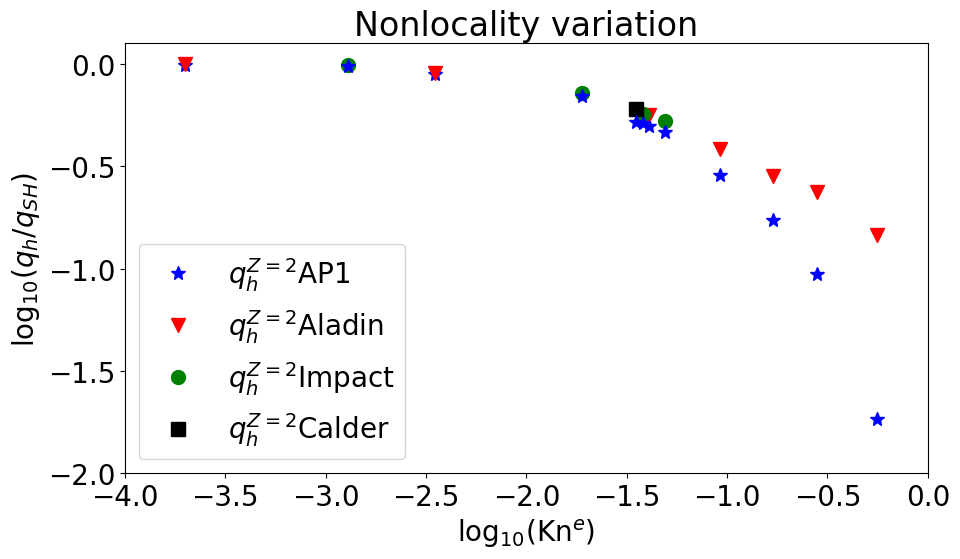
\includegraphics[width=0.5\textwidth]{Kn_results.png}
    \end{tabular}
  \caption{  
  Simulation results for the case $Z=2$ computed by AP1/Aladin/Impact/Calder.
  Every point corresponds to the maximum heat flux in a "tanh" temperature 
  simulation, which can be characterized by Kn. The range of 
  $\log_{10}(\text{Kn})\in (0, -4)$ can be expressed as equivalent 
  to the~electron density approximate range n$_e \in (1e19, 3.5e22)$ of 
  the~50 $\mu$m slope tanh case. In the case of Kn = 0.56, 
  $q_{Aladin} / q_{AP1}\approx 7.9$.}
  \end{center}
  \label{fig:q1s_summary}
\end{figure}

\begin{figure}[tbh]
  \begin{center}
    \begin{tabular}{c}
      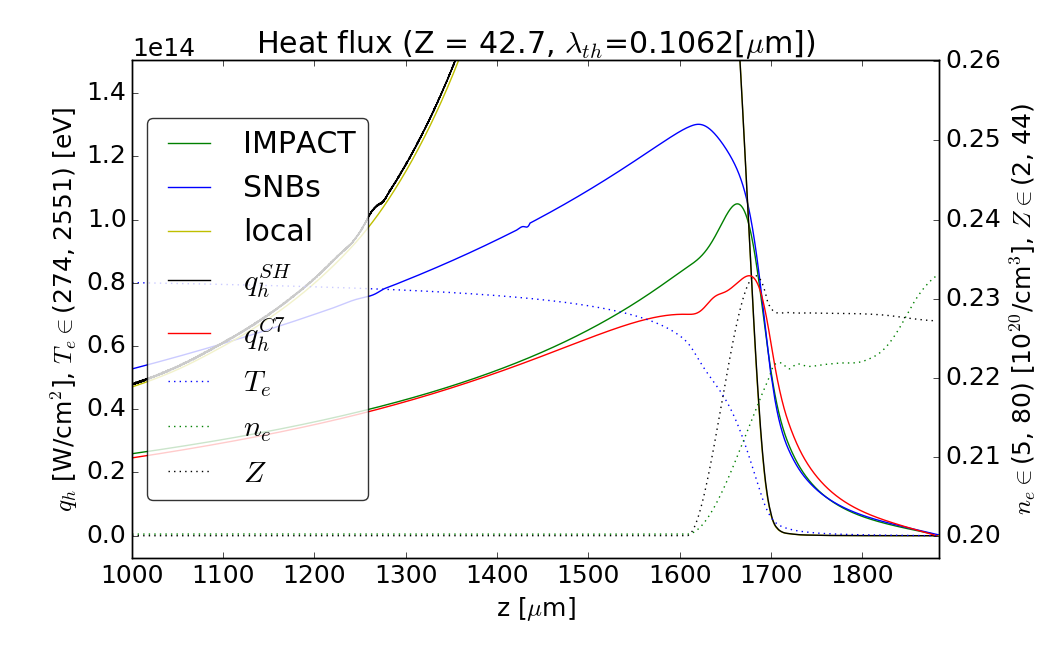
\includegraphics[width=0.5\textwidth]{../VFPdata/GD_Hohlraum/fluxes_10ps.png} 
    \end{tabular}
  \caption{
  }
  \end{center}
  \label{fig:Gd_VFP_10ps_heatflux}
\end{figure}
%\clearpage
